% Options for packages loaded elsewhere
\PassOptionsToPackage{unicode}{hyperref}
\PassOptionsToPackage{hyphens}{url}
\PassOptionsToPackage{dvipsnames,svgnames,x11names}{xcolor}
%
\documentclass[
  11pt,
]{article}

\usepackage{amsmath,amssymb}
\usepackage{setspace}
\usepackage{iftex}
\ifPDFTeX
  \usepackage[T1]{fontenc}
  \usepackage[utf8]{inputenc}
  \usepackage{textcomp} % provide euro and other symbols
\else % if luatex or xetex
  \usepackage{unicode-math}
  \defaultfontfeatures{Scale=MatchLowercase}
  \defaultfontfeatures[\rmfamily]{Ligatures=TeX,Scale=1}
\fi
\usepackage{lmodern}
\ifPDFTeX\else  
    % xetex/luatex font selection
  \setmainfont[]{Arial}
  \setmonofont[]{DejaVu Sans Mono}
\fi
% Use upquote if available, for straight quotes in verbatim environments
\IfFileExists{upquote.sty}{\usepackage{upquote}}{}
\IfFileExists{microtype.sty}{% use microtype if available
  \usepackage[]{microtype}
  \UseMicrotypeSet[protrusion]{basicmath} % disable protrusion for tt fonts
}{}
\makeatletter
\@ifundefined{KOMAClassName}{% if non-KOMA class
  \IfFileExists{parskip.sty}{%
    \usepackage{parskip}
  }{% else
    \setlength{\parindent}{0pt}
    \setlength{\parskip}{6pt plus 2pt minus 1pt}}
}{% if KOMA class
  \KOMAoptions{parskip=half}}
\makeatother
\usepackage{xcolor}
\usepackage[lmargin=0.8in,rmargin=0.8in,tmargin=0.8in,bmargin=0.8in]{geometry}
\ifLuaTeX
  \usepackage{luacolor}
  \usepackage[soul]{lua-ul}
\else
  \usepackage{soul}
  
\fi
\setlength{\emergencystretch}{3em} % prevent overfull lines
\setcounter{secnumdepth}{-\maxdimen} % remove section numbering
% Make \paragraph and \subparagraph free-standing
\ifx\paragraph\undefined\else
  \let\oldparagraph\paragraph
  \renewcommand{\paragraph}[1]{\oldparagraph{#1}\mbox{}}
\fi
\ifx\subparagraph\undefined\else
  \let\oldsubparagraph\subparagraph
  \renewcommand{\subparagraph}[1]{\oldsubparagraph{#1}\mbox{}}
\fi

\usepackage{color}
\usepackage{fancyvrb}
\newcommand{\VerbBar}{|}
\newcommand{\VERB}{\Verb[commandchars=\\\{\}]}
\DefineVerbatimEnvironment{Highlighting}{Verbatim}{commandchars=\\\{\}}
% Add ',fontsize=\small' for more characters per line
\usepackage{framed}
\definecolor{shadecolor}{RGB}{241,243,245}
\newenvironment{Shaded}{\begin{snugshade}}{\end{snugshade}}
\newcommand{\AlertTok}[1]{\textcolor[rgb]{0.68,0.00,0.00}{#1}}
\newcommand{\AnnotationTok}[1]{\textcolor[rgb]{0.37,0.37,0.37}{#1}}
\newcommand{\AttributeTok}[1]{\textcolor[rgb]{0.40,0.45,0.13}{#1}}
\newcommand{\BaseNTok}[1]{\textcolor[rgb]{0.68,0.00,0.00}{#1}}
\newcommand{\BuiltInTok}[1]{\textcolor[rgb]{0.00,0.23,0.31}{#1}}
\newcommand{\CharTok}[1]{\textcolor[rgb]{0.13,0.47,0.30}{#1}}
\newcommand{\CommentTok}[1]{\textcolor[rgb]{0.37,0.37,0.37}{#1}}
\newcommand{\CommentVarTok}[1]{\textcolor[rgb]{0.37,0.37,0.37}{\textit{#1}}}
\newcommand{\ConstantTok}[1]{\textcolor[rgb]{0.56,0.35,0.01}{#1}}
\newcommand{\ControlFlowTok}[1]{\textcolor[rgb]{0.00,0.23,0.31}{#1}}
\newcommand{\DataTypeTok}[1]{\textcolor[rgb]{0.68,0.00,0.00}{#1}}
\newcommand{\DecValTok}[1]{\textcolor[rgb]{0.68,0.00,0.00}{#1}}
\newcommand{\DocumentationTok}[1]{\textcolor[rgb]{0.37,0.37,0.37}{\textit{#1}}}
\newcommand{\ErrorTok}[1]{\textcolor[rgb]{0.68,0.00,0.00}{#1}}
\newcommand{\ExtensionTok}[1]{\textcolor[rgb]{0.00,0.23,0.31}{#1}}
\newcommand{\FloatTok}[1]{\textcolor[rgb]{0.68,0.00,0.00}{#1}}
\newcommand{\FunctionTok}[1]{\textcolor[rgb]{0.28,0.35,0.67}{#1}}
\newcommand{\ImportTok}[1]{\textcolor[rgb]{0.00,0.46,0.62}{#1}}
\newcommand{\InformationTok}[1]{\textcolor[rgb]{0.37,0.37,0.37}{#1}}
\newcommand{\KeywordTok}[1]{\textcolor[rgb]{0.00,0.23,0.31}{#1}}
\newcommand{\NormalTok}[1]{\textcolor[rgb]{0.00,0.23,0.31}{#1}}
\newcommand{\OperatorTok}[1]{\textcolor[rgb]{0.37,0.37,0.37}{#1}}
\newcommand{\OtherTok}[1]{\textcolor[rgb]{0.00,0.23,0.31}{#1}}
\newcommand{\PreprocessorTok}[1]{\textcolor[rgb]{0.68,0.00,0.00}{#1}}
\newcommand{\RegionMarkerTok}[1]{\textcolor[rgb]{0.00,0.23,0.31}{#1}}
\newcommand{\SpecialCharTok}[1]{\textcolor[rgb]{0.37,0.37,0.37}{#1}}
\newcommand{\SpecialStringTok}[1]{\textcolor[rgb]{0.13,0.47,0.30}{#1}}
\newcommand{\StringTok}[1]{\textcolor[rgb]{0.13,0.47,0.30}{#1}}
\newcommand{\VariableTok}[1]{\textcolor[rgb]{0.07,0.07,0.07}{#1}}
\newcommand{\VerbatimStringTok}[1]{\textcolor[rgb]{0.13,0.47,0.30}{#1}}
\newcommand{\WarningTok}[1]{\textcolor[rgb]{0.37,0.37,0.37}{\textit{#1}}}

\providecommand{\tightlist}{%
  \setlength{\itemsep}{0pt}\setlength{\parskip}{0pt}}\usepackage{longtable,booktabs,array}
\usepackage{calc} % for calculating minipage widths
% Correct order of tables after \paragraph or \subparagraph
\usepackage{etoolbox}
\makeatletter
\patchcmd\longtable{\par}{\if@noskipsec\mbox{}\fi\par}{}{}
\makeatother
% Allow footnotes in longtable head/foot
\IfFileExists{footnotehyper.sty}{\usepackage{footnotehyper}}{\usepackage{footnote}}
\makesavenoteenv{longtable}
\usepackage{graphicx}
\makeatletter
\def\maxwidth{\ifdim\Gin@nat@width>\linewidth\linewidth\else\Gin@nat@width\fi}
\def\maxheight{\ifdim\Gin@nat@height>\textheight\textheight\else\Gin@nat@height\fi}
\makeatother
% Scale images if necessary, so that they will not overflow the page
% margins by default, and it is still possible to overwrite the defaults
% using explicit options in \includegraphics[width, height, ...]{}
\setkeys{Gin}{width=\maxwidth,height=\maxheight,keepaspectratio}
% Set default figure placement to htbp
\makeatletter
\def\fps@figure{htbp}
\makeatother
% definitions for citeproc citations
\NewDocumentCommand\citeproctext{}{}
\NewDocumentCommand\citeproc{mm}{%
  \begingroup\def\citeproctext{#2}\cite{#1}\endgroup}
\makeatletter
 % allow citations to break across lines
 \let\@cite@ofmt\@firstofone
 % avoid brackets around text for \cite:
 \def\@biblabel#1{}
 \def\@cite#1#2{{#1\if@tempswa , #2\fi}}
\makeatother
\newlength{\cslhangindent}
\setlength{\cslhangindent}{1.5em}
\newlength{\csllabelwidth}
\setlength{\csllabelwidth}{3em}
\newenvironment{CSLReferences}[2] % #1 hanging-indent, #2 entry-spacing
 {\begin{list}{}{%
  \setlength{\itemindent}{0pt}
  \setlength{\leftmargin}{0pt}
  \setlength{\parsep}{0pt}
  % turn on hanging indent if param 1 is 1
  \ifodd #1
   \setlength{\leftmargin}{\cslhangindent}
   \setlength{\itemindent}{-1\cslhangindent}
  \fi
  % set entry spacing
  \setlength{\itemsep}{#2\baselineskip}}}
 {\end{list}}
\usepackage{calc}
\newcommand{\CSLBlock}[1]{\hfill\break\parbox[t]{\linewidth}{\strut\ignorespaces#1\strut}}
\newcommand{\CSLLeftMargin}[1]{\parbox[t]{\csllabelwidth}{\strut#1\strut}}
\newcommand{\CSLRightInline}[1]{\parbox[t]{\linewidth - \csllabelwidth}{\strut#1\strut}}
\newcommand{\CSLIndent}[1]{\hspace{\cslhangindent}#1}

\usepackage{lineno}
\makeatletter
\@ifpackageloaded{caption}{}{\usepackage{caption}}
\AtBeginDocument{%
\ifdefined\contentsname
  \renewcommand*\contentsname{Table of contents}
\else
  \newcommand\contentsname{Table of contents}
\fi
\ifdefined\listfigurename
  \renewcommand*\listfigurename{List of Figures}
\else
  \newcommand\listfigurename{List of Figures}
\fi
\ifdefined\listtablename
  \renewcommand*\listtablename{List of Tables}
\else
  \newcommand\listtablename{List of Tables}
\fi
\ifdefined\figurename
  \renewcommand*\figurename{Figure}
\else
  \newcommand\figurename{Figure}
\fi
\ifdefined\tablename
  \renewcommand*\tablename{Table}
\else
  \newcommand\tablename{Table}
\fi
}
\@ifpackageloaded{float}{}{\usepackage{float}}
\floatstyle{ruled}
\@ifundefined{c@chapter}{\newfloat{codelisting}{h}{lop}}{\newfloat{codelisting}{h}{lop}[chapter]}
\floatname{codelisting}{Listing}
\newcommand*\listoflistings{\listof{codelisting}{List of Listings}}
\makeatother
\makeatletter
\makeatother
\makeatletter
\@ifpackageloaded{caption}{}{\usepackage{caption}}
\@ifpackageloaded{subcaption}{}{\usepackage{subcaption}}
\makeatother
\ifLuaTeX
  \usepackage{selnolig}  % disable illegal ligatures
\fi
\usepackage{bookmark}

\IfFileExists{xurl.sty}{\usepackage{xurl}}{} % add URL line breaks if available
\urlstyle{same} % disable monospaced font for URLs
\hypersetup{
  pdftitle={Cell-type diversity and connectome of the ctenophore apical organ},
  colorlinks=true,
  linkcolor={blue},
  filecolor={Maroon},
  citecolor={Blue},
  urlcolor={Blue},
  pdfcreator={LaTeX via pandoc}}

\title{Cell-type diversity and connectome of the ctenophore apical
organ}
\author{}
\date{}

\begin{document}
\maketitle

\linenumbers

\setstretch{1.2}
\hfill\break

Kei Jokura\textsuperscript{1,3,*}, Sanja Jasek\textsuperscript{1,2},
Lara Kewalow\textsuperscript{2}, Pawel Burkhardt\textsuperscript{4},
Gáspár Jékely\textsuperscript{1,2,*}\\

\textsuperscript{1}Living Systems Institute, University of Exeter,
Exeter, EX4 4QD, United Kingdom\\
\textsuperscript{2}Heidelberg University, Centre for Organismal Studies
(COS), 69120 Heidelberg, Germany\\
\textsuperscript{3}Exploratory Research Center on Life and Living
Systems (ExCELLS), National Institutes of Natural Sciences, Okazaki,
Japan\\
\textsuperscript{4}Michael Sars Centre, University of Bergen, Norway\\
\textsuperscript{*}Correspondence: jokura@nibb.ac.jp,
gaspar.jekely@cos.uni-heidelberg.de

\subsection{Abstract}\label{abstract}

\textbf{text in bold} \emph{italic} \ul{underline}

\subsection{Introduction}\label{introduction}

First descriptions of AO: (Aronova, 1974)

The lobate ctenophore \emph{Mnemiopsis}

The lithocytes have a large calcium carbonate concretion and\ldots{}
(Tamm, 2014a) Living lithocytes are transported along the balancer cilia
to the tip of the statocyst (Noda and Tamm, 2014) The projections of a
group of bridge cells located on two sides of the apical organ forms an
arch and connects the balancers along the tentacular plane (Tamm and
Tamm, 2002).

The easiest way is to use the command line to add new refs to the .bib
file:

\begin{Shaded}
\begin{Highlighting}[]
\CommentTok{\#curl {-}LH "Accept: application/x{-}bibtex" https://doi.org/10.7554/eLife.91258.1 \textgreater{}\textgreater{} references.bib}
\end{Highlighting}
\end{Shaded}

\subsection{Results}\label{results}

\subsubsection{\texorpdfstring{Volume EM reconstruction of the
\emph{Mnemiopsis} apical
organ}{Volume EM reconstruction of the Mnemiopsis apical organ}}\label{volume-em-reconstruction-of-the-mnemiopsis-apical-organ}

\begin{itemize}
\tightlist
\item
  specimen
\item
  volume, resolution, fixation, quality
\item
  number of sections
\item
  skeletonisation in Catmaid
\item
  number of cells
\item
  general anatomy, regions, quadrants
\end{itemize}

\begin{figure}[H]

{\centering 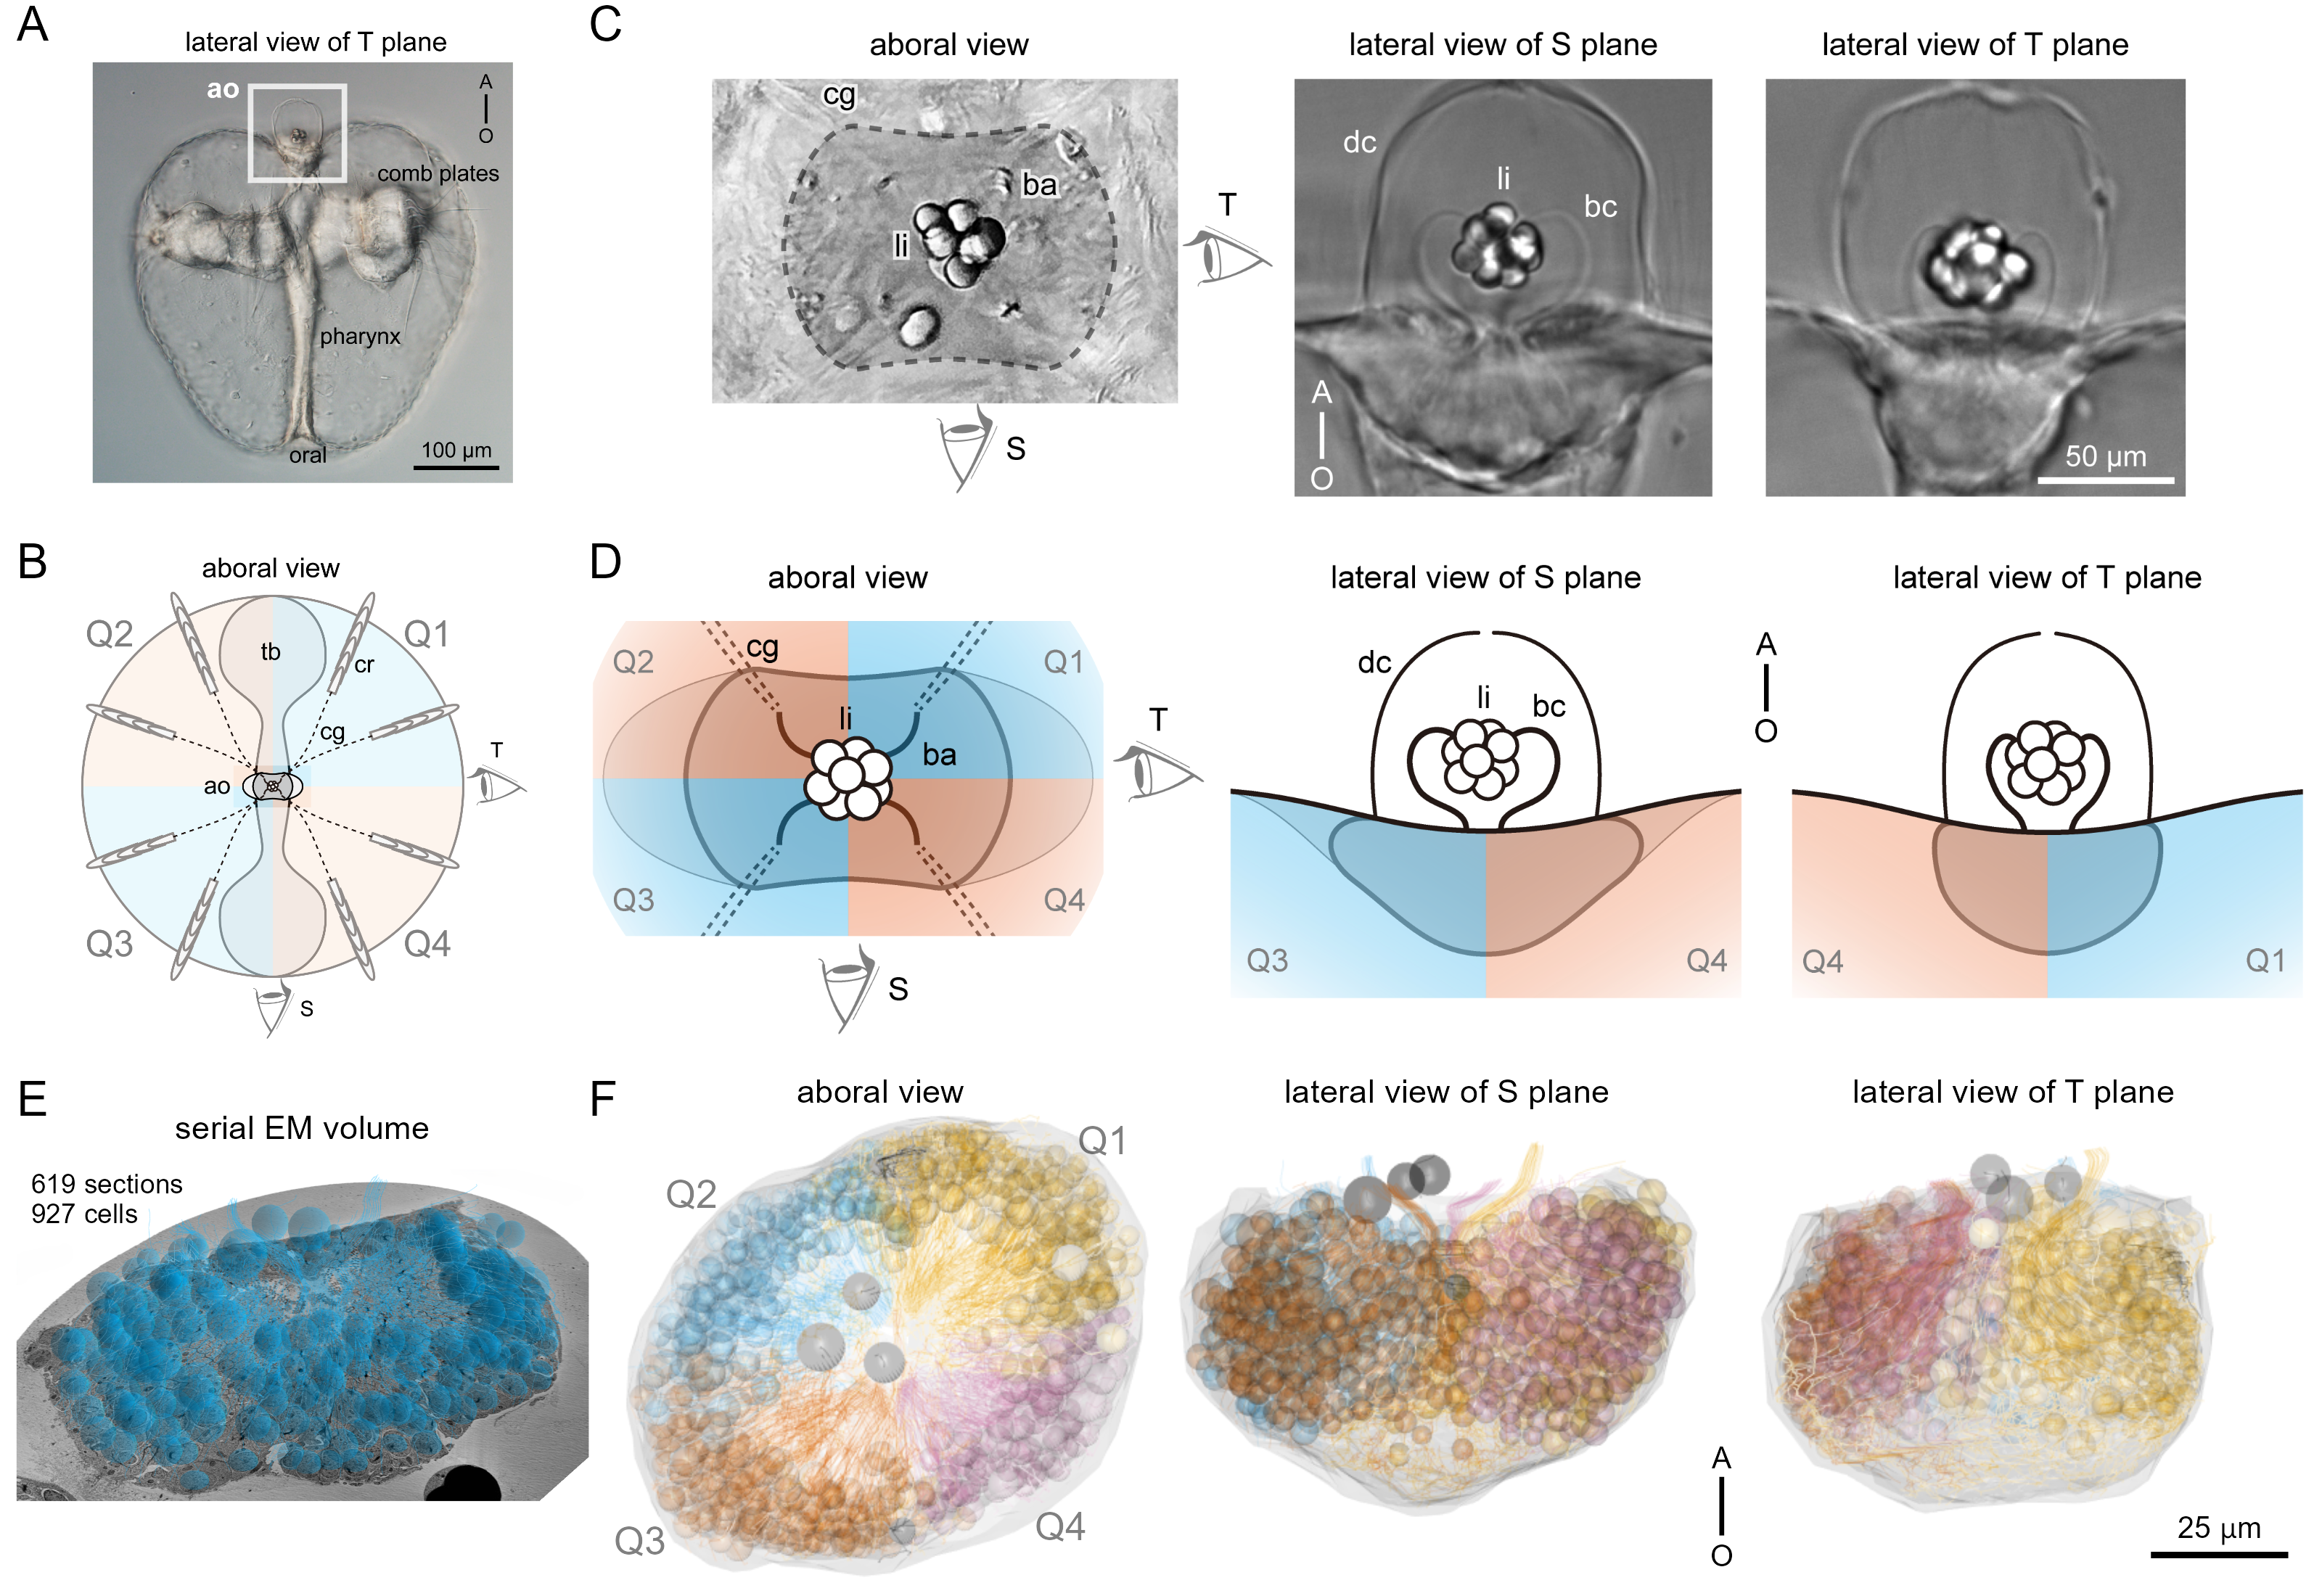
\includegraphics[width=1\textwidth,height=\textheight]{figures/Figure1.png}

}

\caption{\textbf{Figure 1. Title fig 1} pic of a larva, boxed region of
AO, schematic, catmaid pic with slice, dimensions, quadrants, regions,
(A) legend (B) legend.}

\end{figure}%

\subsubsection{Classification of cell
types}\label{classification-of-cell-types}

\begin{itemize}
\tightlist
\item
  ultrastructural criteria (cilia, vesicles etc)
\item
  number of types, cells per type - table
\end{itemize}

\begin{figure}[H]

{\centering 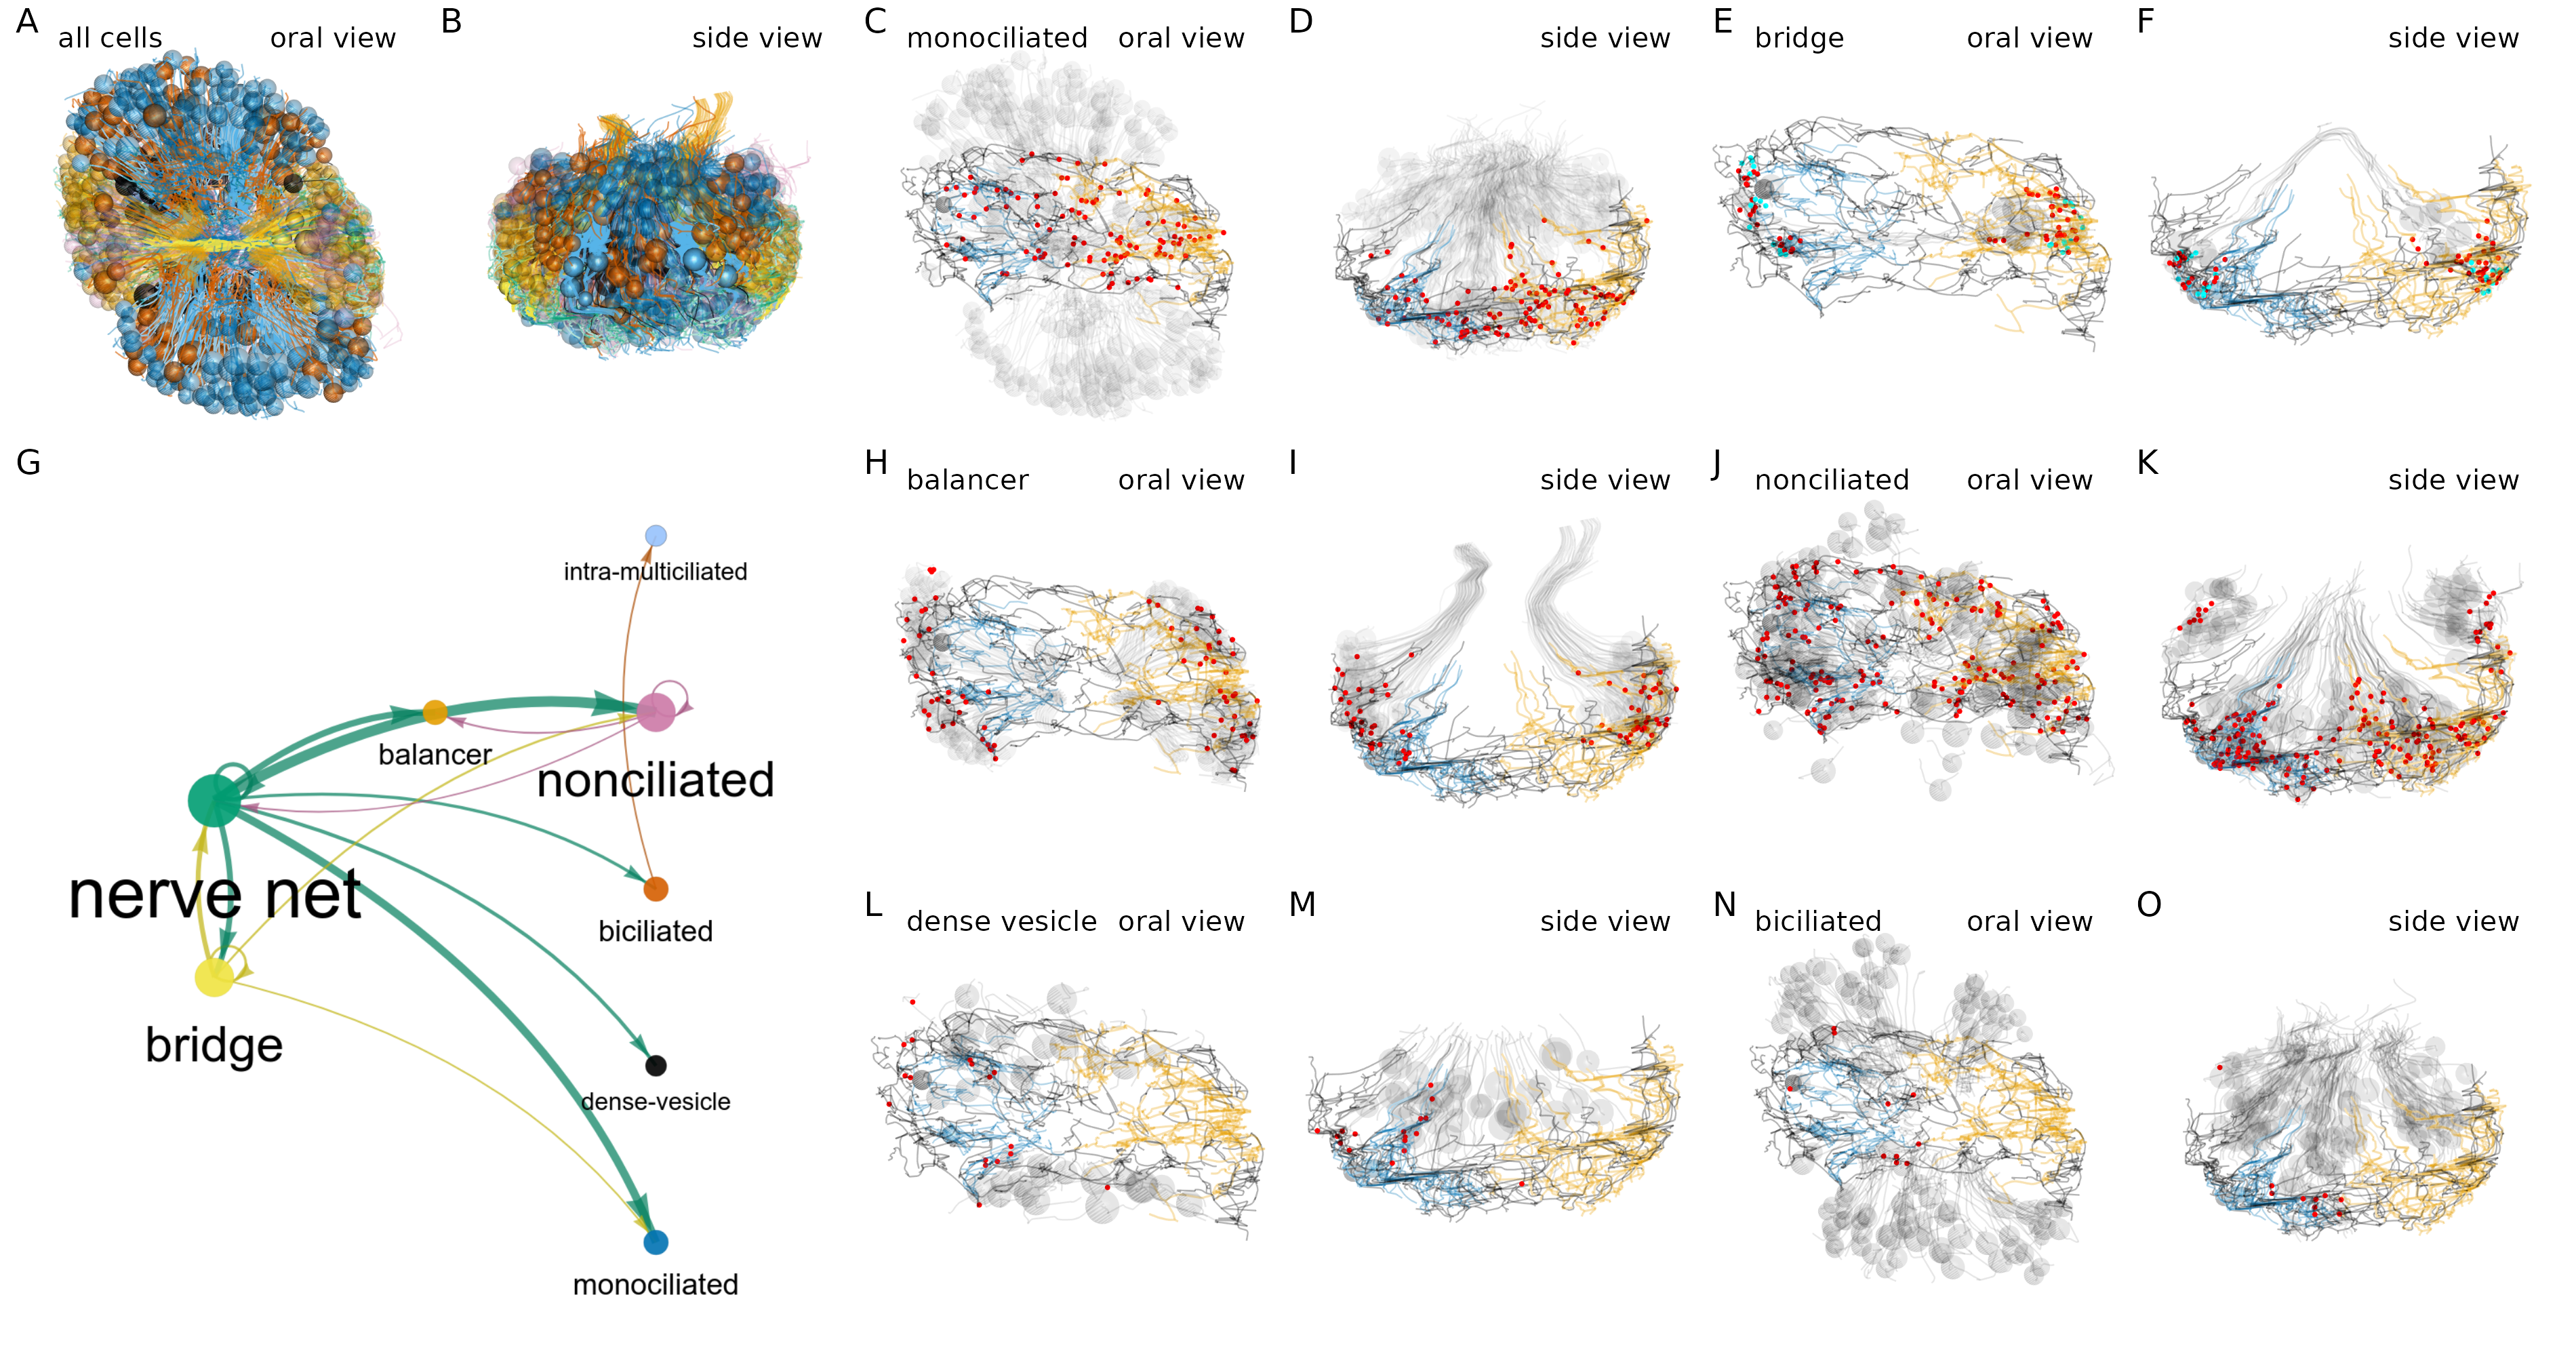
\includegraphics[width=1\textwidth,height=\textheight]{figures/Figure_network.png}

}

\caption{\textbf{Figure 2. Title fig 2} Balancer complex: balancer,
lithocyte, groove 2 types, bridge - EM pics, (A) legend (B) legend.}

\end{figure}%

``the larval bridge has not yet developed forks at its ends, as seen in
adult Mnemiopsis bridges''(Tamm and Tamm, 2002)

Figure3 - dome, bicil, monocil, no-cil, plumose, dense vesicle cells
(rename), gland? cells, oligo/multiciliated cells

Plumose cells (Hernandez-Nicaise, 1984) may be pressure sensors (Tamm,
2014b)

Figure4 - lamellate body complex, LB, intra-multi-ciliated, relationship
to balancer

Figure5 - nerve net, different fragments/cells/syntytia, EM, relation to
entire organ

Figure 6 - cilia? renderings of basal bodies, centrioles, length,
axoneme structure (table), table about cell types, number of cilia etc.

\subsection{Synapses}\label{synapses}

``synaptic regions with the characteristic presynaptic triad mor-
phology of ctenophore nerves (i.e., a single layer of vesicles, smooth
ER sac, and closely apposed mito- chondria (Hernandez-Nicaise, 1973;
Horridge and Mackay, 1964) Hernandez- Nicaise, 1973)''

Figure 7 - synapses, reconstruction, annotation, numbers, distribution
of partners, example EM (figure supplement - lots of EM), mitochondria
(Fig suppl - mitochondrion stats - Sanja)

Gap juntions? Innexins are expressed in the apical organ in specific
patches of cells in each quadrant (Ortiz et al., 2023)

Ctenophore synapses (Hernandez-Nicaise, 1973)

We found no synapses between bridge and balancer, in agreement with Tamm
(Tamm and Tamm, 2002).

Figure 8 - connectome cell-type based, quadrant based, nerve net
syntycia, bridge, quadrants (Fig suppl - cell-based network)

Tamm\&Tamm observed synapses from neurites to bridge cells (2002). and
in Mnemiopsis larvae observed synapses from bridge cells onto other
cells

Inserting Figures

You can add your figures into the rendered document. We saved the
figures into /manuscript/figures or /manuscript/figure\_supplements and
can insert them from there. We use knitr::include\_graphics for this.
The title and legend can also be edited, as will as the width of the
output figure.

\subsection{Equations}\label{equations}

Equations can also be inserted, Insert -\textgreater{} Display Math:

\[
\bar{X} = \frac{\sum_{i=1}^{n} x_{i}}{n}
\]

\subsection{Sourcing code and working with
variable}\label{sourcing-code-and-working-with-variable}

The `analysis/scripts/statistics\_for\_paper.R' script is sourced and it
runs but the output is not included in the knitted output. But we can
access the variables defined in the sourced script simply by adding ` r
var\_name ` between ` backticks, in this case max\_PRC value is (now
this number comes from our sourced script).

If we update the data, the script can recalculate the variable we want
to refer to in the text and update the number.

\subsection{Materials and Methods}\label{materials-and-methods}

\subsection{Acknowledgements}\label{acknowledgements}

We would like to thank the Jekely lab for the R project template
(\url{https://github.com/JekelyLab/new_paper_template}) we used to write
this paper. This work was funded by \ldots{} JSPS\ldots{} ERC.. Others
\ldots{}

\subsection{References}\label{references}

\phantomsection\label{refs}
\begin{CSLReferences}{1}{0}
\bibitem[\citeproctext]{ref-aronova1974electron}
Aronova M. 1974. Electron microscopic observation of the aboral organ of
ctenophora. I. The gravity receptor. \emph{Zeitschrift fur
mikroskopisch-anatomische Forschung} \textbf{88}:401--412.

\bibitem[\citeproctext]{ref-Hernandez_Nicaise_1984}
Hernandez-Nicaise M-L. 1984. CtenophoraBiology of the Integument.
Springer Berlin Heidelberg. pp. 96--111.
doi:\href{https://doi.org/10.1007/978-3-642-51593-4_9}{10.1007/978-3-642-51593-4\_9}

\bibitem[\citeproctext]{ref-Hernandez_Nicaise_1973}
Hernandez-Nicaise M-L. 1973. The nervous system of ctenophores III.
Ultrastructure of synapses. \emph{Journal of Neurocytology}
\textbf{2}:249--263.
doi:\href{https://doi.org/10.1007/bf01104029}{10.1007/bf01104029}

\bibitem[\citeproctext]{ref-Horridge_1964}
Horridge GA, Mackay B. 1964. Neurociliary synapses in pleurobrachia
(ctenophora). \emph{Journal of Cell Science} \textbf{S3-105}:163--174.
doi:\href{https://doi.org/10.1242/jcs.s3-105.70.163}{10.1242/jcs.s3-105.70.163}

\bibitem[\citeproctext]{ref-Noda_2014}
Noda N, Tamm SL. 2014. Lithocytes are transported along the ciliary
surface to build the statolith of ctenophores. \emph{Current Biology}
\textbf{24}:R951--R952.
doi:\href{https://doi.org/10.1016/j.cub.2014.08.045}{10.1016/j.cub.2014.08.045}

\bibitem[\citeproctext]{ref-Ortiz_2023}
Ortiz J, Bobkov YV, DeBiasse MB, Mitchell DG, Edgar A, Martindale MQ,
Moss AG, Babonis LS, Ryan JF. 2023. Independent innexin radiation shaped
signaling in ctenophores. \emph{Molecular Biology and Evolution}
\textbf{40}.
doi:\href{https://doi.org/10.1093/molbev/msad025}{10.1093/molbev/msad025}

\bibitem[\citeproctext]{ref-Tamm_2014}
Tamm SL. 2014a. Formation of the statolith in the ctenophore mnemiopsis
leidyi. \emph{The Biological Bulletin} \textbf{227}:7--18.
doi:\href{https://doi.org/10.1086/bblv227n1p7}{10.1086/bblv227n1p7}

\bibitem[\citeproctext]{ref-Tamm_2014b}
Tamm SL. 2014b. Cilia and the life of ctenophores. \emph{Invertebrate
Biology} \textbf{133}:1--46.
doi:\href{https://doi.org/10.1111/ivb.12042}{10.1111/ivb.12042}

\bibitem[\citeproctext]{ref-Tamm_2002}
Tamm SL, Tamm S. 2002. Novel bridge of axon‐like processes of epithelial
cells in the aboral sense organ of ctenophores. \emph{Journal of
Morphology} \textbf{254}:99--120.
doi:\href{https://doi.org/10.1002/jmor.10019}{10.1002/jmor.10019}

\end{CSLReferences}



\end{document}
